% Section des résultat: Application sur des réseaux biologiques

The time complexities estimated from the results of computational experiments are a little different from those obtained by theoretical analysis. \Maxime{Qu'est-ce que la phrase précédente signifie ? Qu'entend-on par “theoretical analysis” ?} However, this is reasonable since, in our theoretical analysis, we assumed that the number of genes is very large.
%In this section, we. 
All experiments were run on a PC with Pentium VII 3 GHz processor and 16 Go memory.

\subsection{Lambda Phage model}
\begin{figure}[h]
   \caption{\label{fig:lambda-graph} 
   The figures are taken from \cite{thieffry1995dynamical,chaouiya2008petri} of the Lambda phage model. The left one presents the regulatory graph with positive and negative regulations represented by ’$+$’ and ’$-$’ signs. The second is the corresponding state transition graph (STG).% colored according to strongly connected components. 
We have two attractors: $(2000)$ is an attractor of size $1$ i.e a fixed point and $\{(0300), (0200)\}$ is an attractor of size $2$.}
   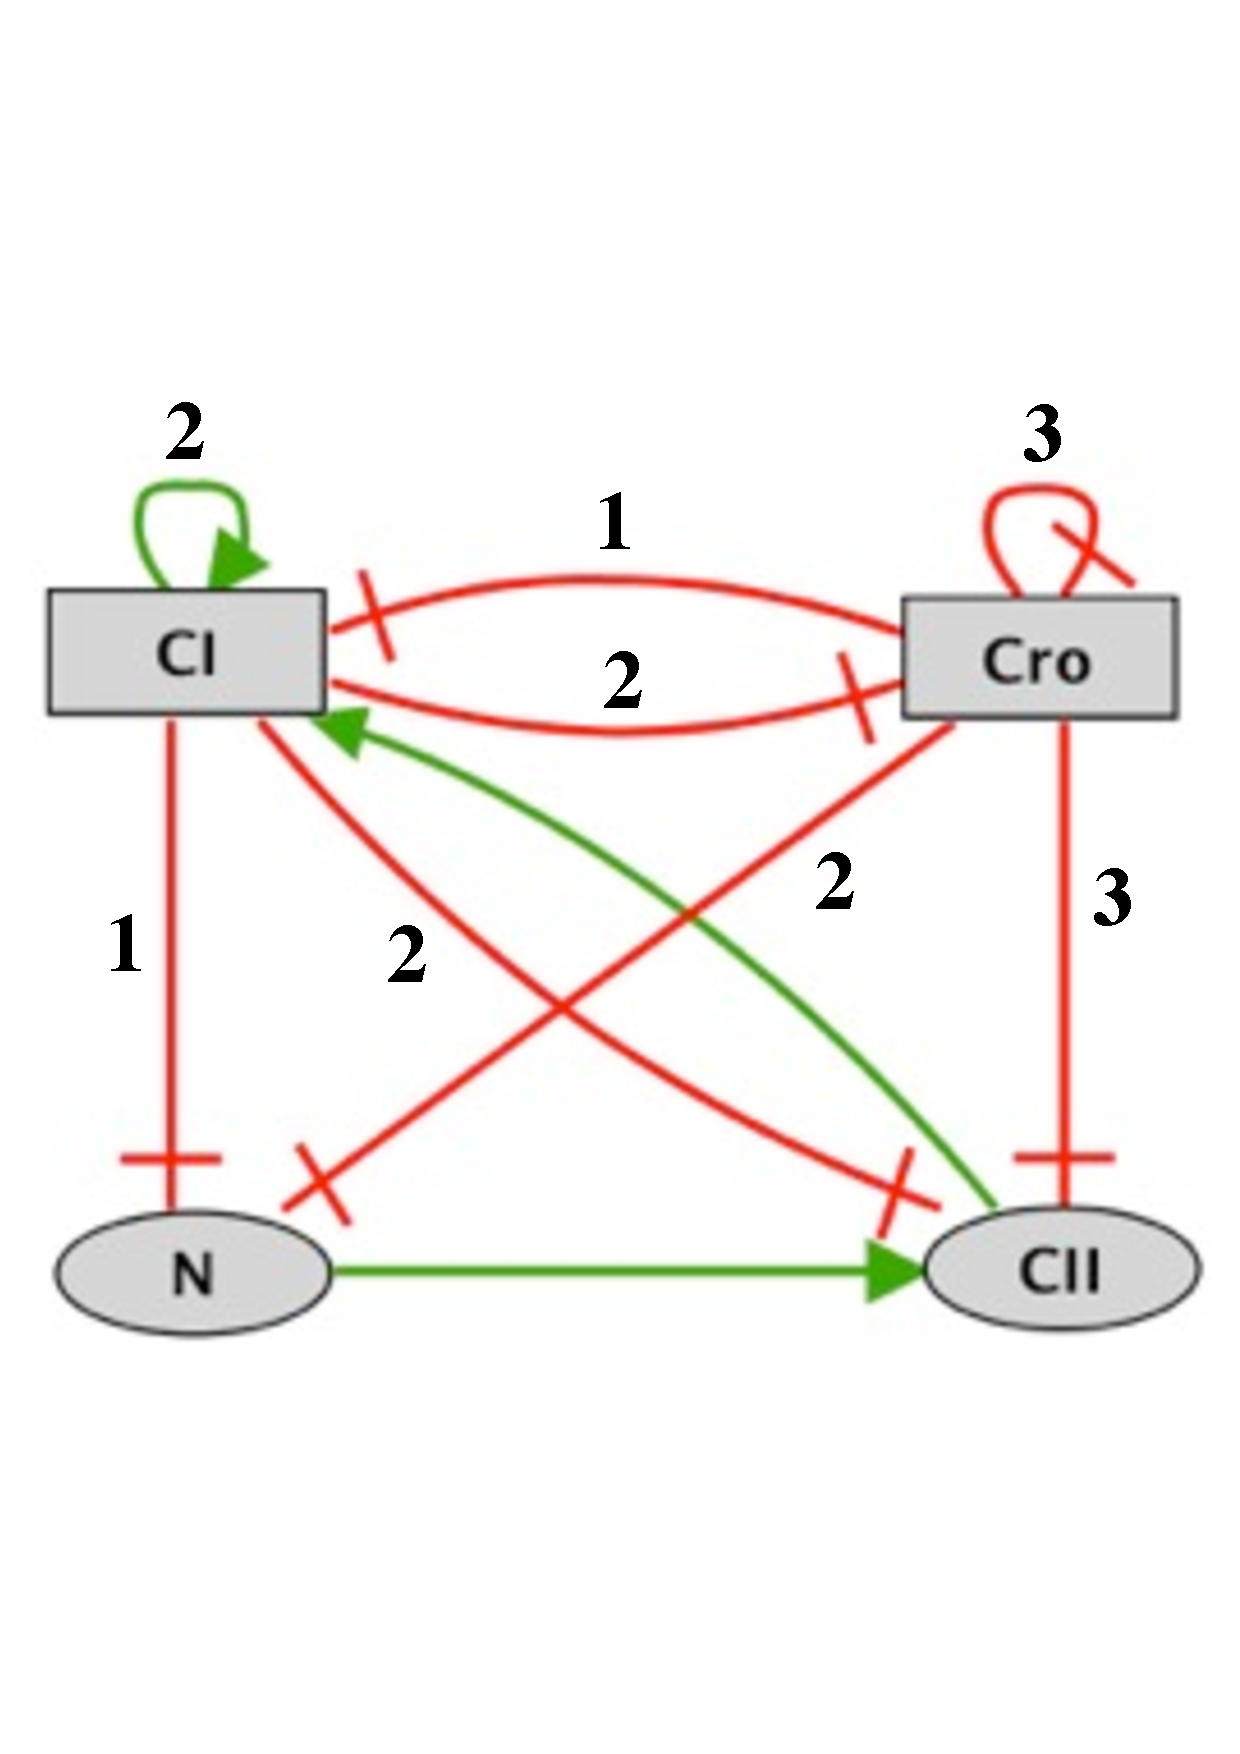
\includegraphics{figures/lampdaphage-thomas.pdf}
   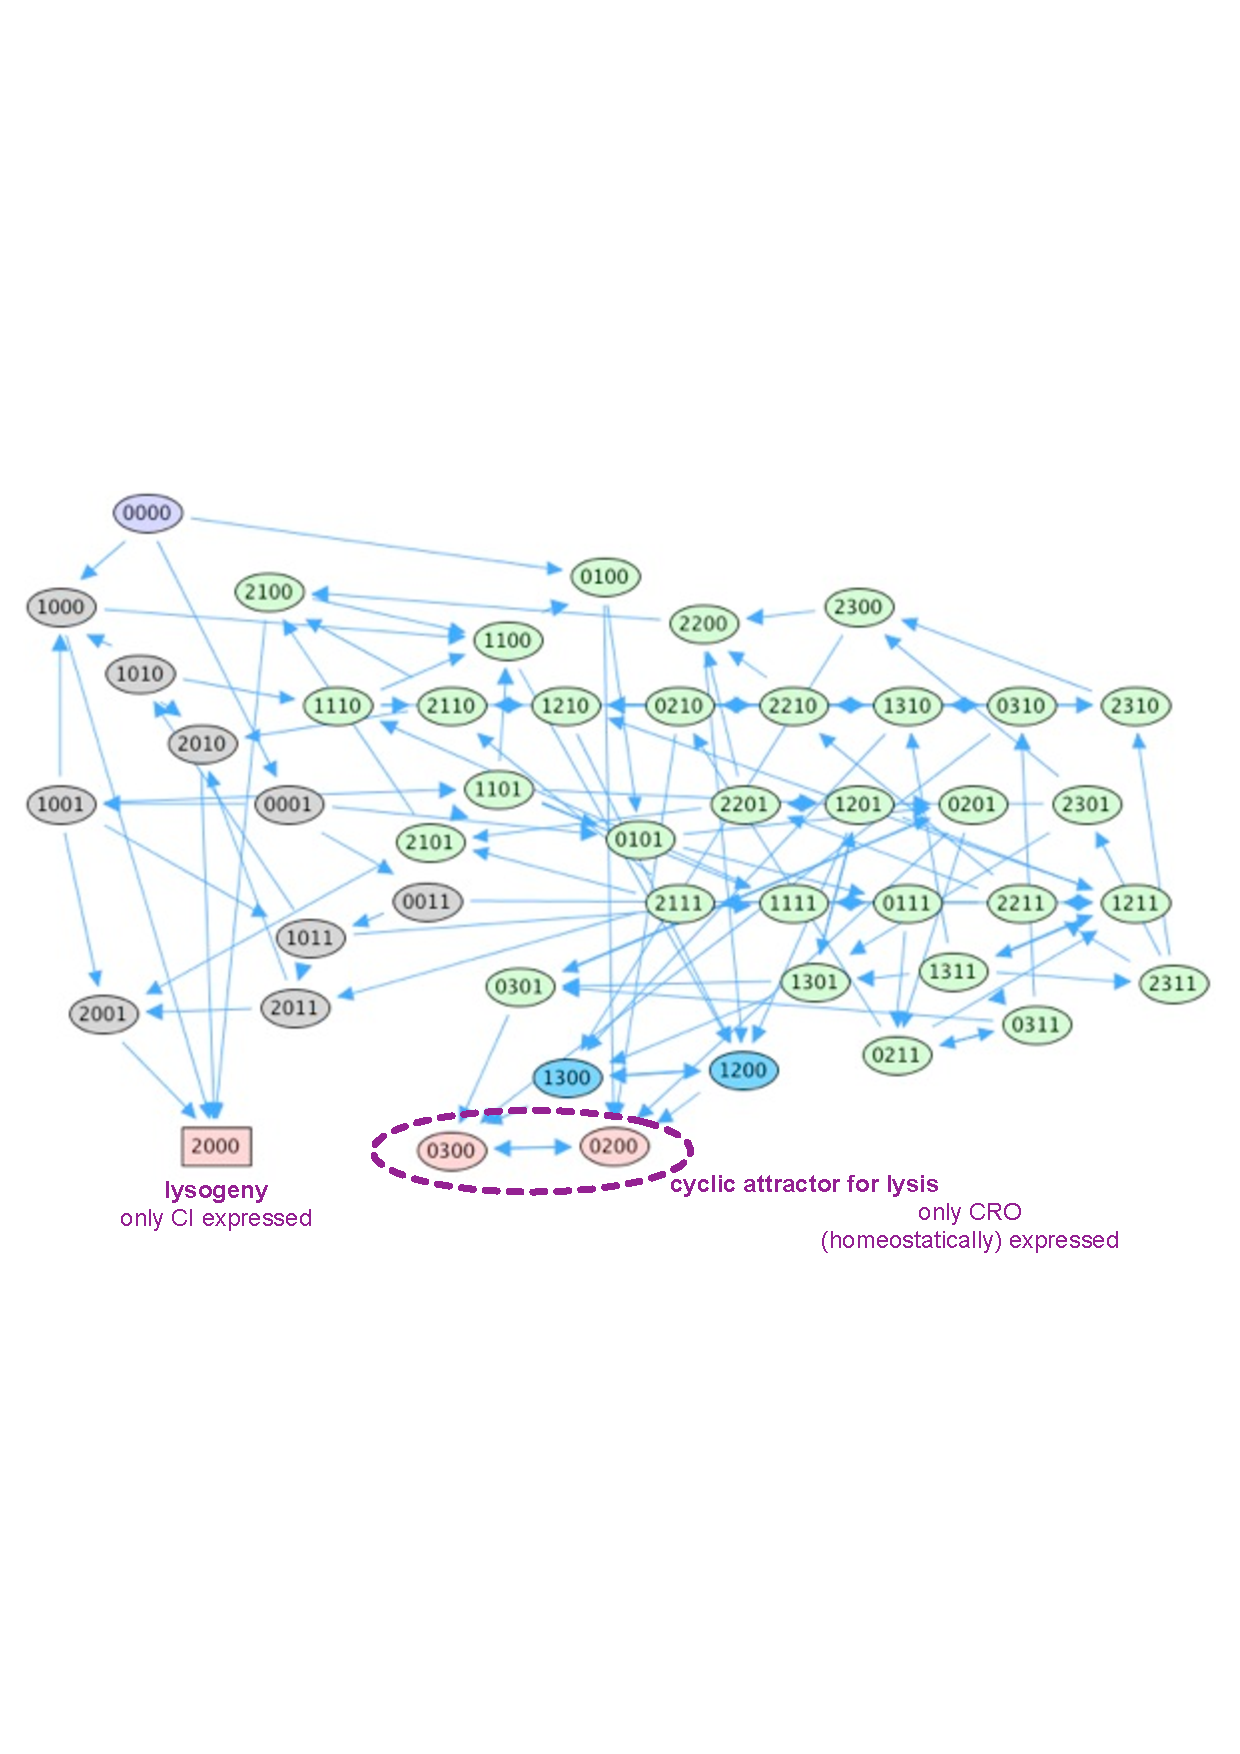
\includegraphics{figures/lampdaphage-STG.pdf}
\end{figure}

Like mentioned above, using our method we are not obliged to have the whole State Transition Graph. So that for finding these attractors (size $1$ and size $2$), it sufficient to compute only graphs of size $2$.
\Maxime{Ici, il faudrait répéter certains éléments de la description de la Figure 3 pour une meilleure compréhension.}

This network was modeled into an Automata Network ($4$ sorts, $48$ processes and $49$ actions) to be analysed later. The result that we get are the following: \\
\textit{ Lambda Phage Fixed points:} $\PHstate{CI_2, CII_0, Cro_0, N_0}$
\begin{lstlisting}[numbers=none]
Answer: 1
selectProc("CI",2) selectProc("CII",0) selectProc("Cro",0) selectProc("N",0)
\end{lstlisting}
\textit{Lambda Phage attractors of size $2$:} \{$\PHstate{CI_0, CII_0, Cro_2, N_0}$, $\PHstate{CI_0, CII_0, Cro_3, N_0}$ \}
\begin{lstlisting}[numbers=none]
Answer: 1
selectProcSt(activeProc("CI",0),0) selectProcSt(activeProc("CII",0),0)
selectProcSt(activeProc("Cro",2),0) selectProcSt(activeProc("N",0),0) 
selectProcSt(activeProc("CI",0),1) selectProcSt(activeProc("CII",0),1)
selectProcSt(activeProc("Cro",3),1) selectProcSt(activeProc("N",0),1)
 \end{lstlisting}

Thus we obtain $1$ answer set for each size that match the expected results. The program needed only $10$ms for finding the fixed point and $19$ms for the attractor.

\subsection{Benchmarks}
As benchmarks we use existing Multi-valued networks models of real organisms shown in Table \ref{tab:models}\benchmarksfootnote: the bacteriophage lambda phage \cite{thieffry1995dynamical}, the Hedgehog Signalling Pathway (\Emna{à revoir la réf} \cite{stecca2010context}), mTOR pathway in survival mechanisms \cite{javle2010inhibition} (\Emna{en cours de traduction}) and egf-tnf which is a mammalian signalling pathways induced by the Epidermal Growth Factor (EGF) and Tumour Necrosis Factor alpha (TNF$\alpha$) \cite{chaouiya2013sbml}.
We have constructed the input descriptions of these models, the automata networks, manually from the data in the corresponding papers.

\begin{changemargin}{-3cm}{-3cm}
\begin{center}
\begin{table*}[ht]
\begin{center}
\noindent%
%\begin{tabular}{| l| c | c | c ||>{\columncolor{verylightgray}} c | c ||>{\columncolor{verylightgray}}c | c | c ||}
\begin{tabular}{| l || c | c | c || c | c || c | c | c |}
\hline
\multicolumn{1}{| l ||}{Models} & \multicolumn{3}{c||}{PH representation} & \multicolumn{2}{c||}{Fixed points} & \multicolumn{3}{c|}{Attractors}\\
\hline
    & sorts & processes & states & sec &  \#results & sec & size & \#results \\
\hline
\hline
%  TTR  & 12 & 42  & $2^{19}$ & 0.004 & 0 & 0.004 & k & 0\\
%\hline
%  ERBB & 42 & 152 & $2^{70}$ & 0.017 & 3 & 0.004 & k & 0\\
%\hline
%  TCR & 54 & 156 & $2^{73}$ & 0.021 & 1 & 0.004 & k & 0\\
%\hline  
   \multirow{3}{*}{lambdaPhage}  & \multirow{3}{*}{4} & \multirow{3}{*}{11} & \multirow{3}{*}{48} & \multirow{3}{*}{0.003} & \multirow{3}{*}{1} & 0.019 & 2 & 1\\
 & & & & & & 0.033 & 4 & 0\\
 & & & & & & 0.470 & 20 & 0\\

\hline
 \multirow{3}{*}{hedgehog}  & \multirow{3}{*}{5} & \multirow{3}{*}{11} & \multirow{3}{*}{48} & \multirow{3}{*}{0.003} & \multirow{3}{*}{2} & 0.017 & 2 & 0\\
 & & & & & & 0.050 & 6 & 0\\
 & & & & & & 0.319 & 20 & 0\\
\hline
 \multirow{3}{*}{mTOR}  & \multirow{3}{*}{6} & \multirow{3}{*}{12} & \multirow{3}{*}{$2^6$} & \multirow{3}{*}{-} & \multirow{3}{*}{-} & - & - & -\\
 & & & & & & - & - & -\\
 & & & & & & - & - & -\\
\hline
 \multirow{3}{*}{egf-tnf}  & \multirow{3}{*}{28} & \multirow{3}{*}{56} & \multirow{3}{*}{$2^{28}$} & \multirow{3}{*}{0.005} & \multirow{3}{*}{2} & 0 & 2 & 0\\
 & & & & & & 9.192 & 8 & 1\\
% & & & & & & xxx & xx & x\\
\hline
\end{tabular}
\vspace*{4pt}
\caption{\label{tab:models}%
Description of the models used in our tests and results of fixed points and attractors enumeration.
Each model is referred to by its short name, where
lambdaPhage stands for the bacteriophage lambda phage \cite{thieffry1995dynamical}, hedgehog for the Hedgehog Signalling Pathway \cite{stecca2010context}, mTOR for the pathway in survival mechanisms \cite{javle2010inhibition} and egf-tnf for the mammalian signalling pathways induced by the Epidermal Growth Factor (EGF) and Tumour Necrosis Factor alpha (TNF$\alpha$) \cite{chaouiya2013sbml}.
For each of them, this table gives the number of biological components
in the original representation,
and the number of sorts, the number of processes
and the number of states in the PH model.
Then, the next two columns give the computation time for the enumeration of all fixed points and the number of results returned. Finally, the last three columns give the computation time for the enumeration of all attractors, their size and the number of found attractors for each size.
}
\end{center}
\end{table*}
\end{center}
\end{changemargin}
